\documentclass[11pt,a4paper]{article}
\usepackage[T1]{fontenc}
\usepackage[utf8]{inputenc}
\usepackage{lmodern}
\usepackage[margin=25mm]{geometry}
\usepackage{microtype,amsmath,amssymb,booktabs,tabularx,array}
\usepackage{tikz}
\usetikzlibrary{arrows.meta,positioning,fit,backgrounds}
\usepackage[section]{placeins}
\usepackage{graphicx}
\usepackage[font=small,labelfont=bf]{caption}
\raggedbottom
\clubpenalty=10000
\widowpenalty=10000
\displaywidowpenalty=10000
\renewcommand{\topfraction}{0.9}
\renewcommand{\bottomfraction}{0.8}
\renewcommand{\textfraction}{0.08}
\renewcommand{\floatpagefraction}{0.8}
\setlength{\floatsep}{12pt}
\setlength{\textfloatsep}{14pt}
\setlength{\intextsep}{12pt}
\makeatletter
\setlength{\@fptop}{0pt}
\setlength{\@fpsep}{16pt}
\makeatother
\definecolor{studyblue}{HTML}{0072B2}
\definecolor{studyorange}{HTML}{D55E00}
\definecolor{studygreen}{HTML}{009E73}
\tikzset{box/.style={draw=studyblue!75,fill=studyblue!5,rounded corners=2pt,align=center,inner sep=7pt,font=\small},arrow/.style={-{Stealth[length=2mm]},thick,draw=black!65},note/.style={font=\small,align=center}}
\usepackage[numbers,sort&compress]{natbib}
\usepackage[colorlinks=true,linkcolor=blue,citecolor=blue,urlcolor=blue]{hyperref}
\setlength{\parskip}{3pt}
\setlength{\parindent}{1em}
\newcolumntype{Y}{>{\raggedright\arraybackslash}X}
\title{Repository Organization and Behavioral Verification\\for Agent-Driven SaaS Feature Extension}
\author{Do Hoang Trieu\\Vietnamese--German University}
\date{}
\begin{document}
\maketitle
\begin{abstract}
Extending an existing application requires a coding agent to implement new behavior while preserving requirements that remain in force. A starter kit can influence this process through the organization of its code and the checks available during implementation. We propose a controlled study of these two design choices using SmartKit, a Next.js SaaS starter kit developed in a preceding bachelor thesis. A $2\times2$ design will compare feature-based and layer-based organization, each with and without an additional behavioral verification package. All conditions will share task requirements, initial application behavior, and execution budgets. Independent acceptance and preservation checks will determine joint success; component outcomes and execution costs will be reported separately. The study will qualify matched repository variants, validate task-specific evaluators, and use a separate development pilot before freezing the main protocol. No new experimental results are reported. The intended contribution is evidence about specific starter-kit interventions and their limits, supported by traceable tasks and reproducible run artifacts.
\end{abstract}

\section{Introduction}
Consider a request to add order search to an existing SaaS application. An implementation could return the requested orders and still expose records belonging to another user if the change omits an ownership restriction. Figure~\ref{fig:motivation} illustrates this hypothetical example, not an observed SmartKit incident. Evaluating a feature change requires both acceptance criteria for the new functionality and checks for existing requirements that the change must preserve.

\begin{figure}[htbp]
\centering
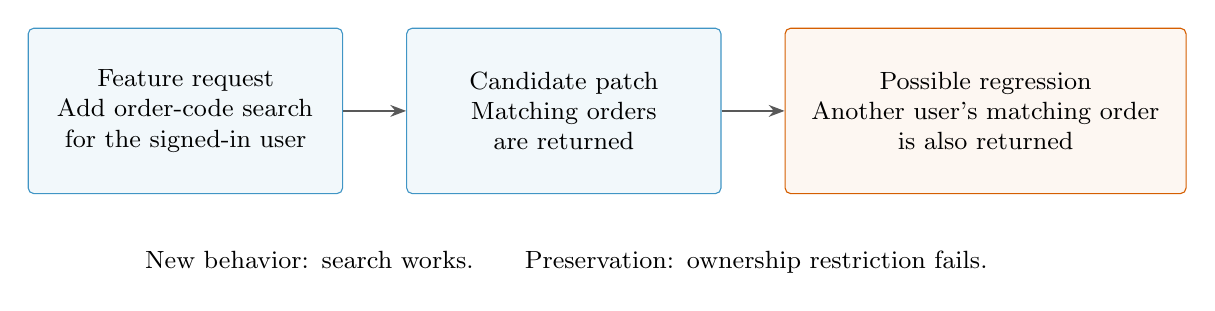
\begin{tikzpicture}[node distance=8mm]
\node[box,text width=3.5cm,minimum height=21mm] (request) {Feature request\\Add order-code search\\for the signed-in user};
\node[box,right=of request,text width=3.5cm,minimum height=21mm] (patch) {Candidate patch\\Matching orders\\are returned};
\node[box,right=of patch,text width=4.6cm,minimum height=21mm,draw=studyorange,fill=studyorange!5] (risk) {Possible regression\\Another user's matching order\\is also returned};
\draw[arrow] (request)--(patch);
\draw[arrow] (patch)--(risk);
\node[note,below=6mm of patch,text width=12cm] {New behavior: search works.\qquad Preservation: ownership restriction fails.};
\end{tikzpicture}
\caption{Hypothetical order-search extension with an ownership regression.}
\label{fig:motivation}
\end{figure}


Repository-level evaluation makes this distinction operational. SWE-bench asks systems to modify real repositories from issue descriptions and evaluates the resulting patches~\cite{jimenez2024swebench}; SWE-Bench Pro broadens the setting to longer, multi-file engineering tasks~\cite{deng2025swepro}. These benchmarks establish realistic task settings, while our proposed intervention study asks how alternative organizations of the same application affect behavior under matched requirements.

The preceding thesis developed SmartKit, a Next.js starter kit with authentication, billing, and email components, and examined coding-assistant adherence to repository conventions~\cite{trieu2026thesis}. Its evaluation emphasized artifacts such as file placement, type and schema usage, and required components. These measurements address whether generated code follows the intended conventions. They leave a separate question: do specific starter-kit design choices help an agent complete a change without introducing regressions?

Recent work makes this question more precise. Repository instructions do not consistently improve task success across evaluated settings~\cite{gloaguen2026agents}. Existing code and its placement can influence agents' implementation decisions~\cite{zhu2026precedent}. Structural requirements have also been evaluated alongside executable behavior in backend generation~\cite{dente2026constraint}. Consequently, a comparison that bundles SmartKit's layout, instructions, examples, and tests would provide limited evidence about which design choice caused an observed difference.

We propose manipulating repository organization and access to an additional behavioral verification package within the same application. The central outcome is joint success: a patch satisfies the requested behavior and preserves the applicable existing behavior under an independent evaluator. This formulation permits feature completion and preservation to fail separately and avoids treating compliance with the author's preferred paths as evidence of correctness.

The planned study has two research products: a matched comparison of concrete repository and verification interventions, and an auditable collection of tasks, evaluators, and agent traces. Their scientific value depends on baseline qualification and comparison with the closest prior artifacts. We make no claim of priority for studying repository layout, tests, or joint correctness. The initial scope is a controlled SmartKit case study; broader claims require independent replication.

\section{Related work}
\subsection{Repository-level agents and patch evaluation}
SWE-agent studies the interface through which a model navigates files, edits code, and executes programs~\cite{yang2024sweagent}. Agentless separates localization, repair, and patch validation, showing that a simpler workflow is a meaningful comparator~\cite{xia2024agentless}. Together with SWE-bench and SWE-Bench Pro~\cite{jimenez2024swebench,deng2025swepro}, these studies motivate treating the harness, task specification, and execution environment as part of the evaluated system. We will hold them fixed when estimating repository interventions. We do not propose a new agent architecture or infer that a more complex workflow must perform better.

\subsection{Repository context and implementation choices}
Parnas's account of modular decomposition connects module boundaries to the design decisions they hide and the changes they localize~\cite{parnas1972modules}. This provides a rationale for examining change locality, but does not establish that feature folders improve agent performance. Moreover, feature-based grouping alone does not demonstrate information hiding. Our comparison manipulates a concrete source organization while preserving the checked application contracts.

Gloaguen et al. distinguish LLM-generated from developer-written context files: generated files generally reduced resolution rates, while developer-written files had a small positive average difference from no context that was not statistically significant in their reported comparison~\cite{gloaguen2026agents}. This mixed evidence supports controlling instruction exposure, not assuming that all repository guidance is ineffective. Zhu et al. manipulate repository precedents and task instructions; their results show that placement can affect implementation choice~\cite{zhu2026precedent}. Their local-versus-sibling comparison also changes task relatedness, so it does not isolate proximity alone. Our organization intervention similarly includes changes to locality, imports, and traversal exposure.

Context exposure also has a broader precedent. Liu et al. show positional sensitivity in long-context question answering and retrieval~\cite{liu2024lost}. Those tasks differ from repository editing, so their findings motivate logging exposure and traversal rather than predicting an organization effect. The direct repository-level evidence remains the relevant basis for the proposed comparison.

\subsection{Constraints and downstream software evolution}
Constraint Decay evaluates backend tasks using behavioral tests and static verifiers, finding that accumulated structural requirements can reduce performance~\cite{dente2026constraint}. Thus, evaluating functionality together with constraints is already established. Our candidate extension concerns matched starter-kit variants and preservation during feature changes.

CodeThread compares subsequent agent performance on human and agent implementations and finds that traditional maintainability metrics do not fully explain downstream differences~\cite{patel2026codethread}. This supports evaluating later behavior directly, but provides no direct estimate of the proposed layout intervention. Evidence from human maintenance also needs separate interpretation: Borg et al. find no systematic downstream maintainability advantage or disadvantage in their human software-evolution setting~\cite{borg2026echoes}. Our study measures autonomous agent performance under fixed budgets, not developer productivity or human maintenance effort.

FeatureArc evaluates successive extensions of a feature in a persistent agent session, using checks for new and existing behavior~\cite{wang2026featurearc}. Its preservation endpoint is close to ours. Our intended distinction is a matched organization-by-verification intervention on fresh sessions, rather than a benchmark of accumulated multi-stage changes. Separately, Mehta studies controlled changes to agents' verification tools when building web applications~\cite{mehta2026verification}. Our package targets specified preservation behavior during extension of an existing application. Both are recent preprints; the final novelty claim still requires comparing their artifacts with our implemented conditions.

\subsection{Validity of executable evaluation}
The test-oracle problem concerns deciding whether observed behavior is correct, with specifications, contracts, and domain knowledge providing possible evidence~\cite{barr2015oracle}. Executing more tests does not by itself resolve that problem. EvalPlus demonstrates that strengthening code-generation test suites can expose previously undetected incorrect programs and change model rankings~\cite{liu2023evalplus}. Our evaluator therefore needs a defensible requirement basis and qualification against valid and faulty implementations.

Inozemtseva and Holmes find low to moderate coverage--effectiveness correlations after controlling test-suite size in their Java study~\cite{inozemtseva2014coverage}. Just et al. report a relationship between mutant detection and real-fault detection in their evaluated systems~\cite{just2014mutants}, while Zhao et al. show that the usefulness of coverage and mutation scores for LLM-generated tests depends on the testing setting~\cite{zhao2026coverage}. These findings support using mutation checks as diagnostic evidence with stated limits. They do not justify replacing behavioral contracts with a coverage target.

Feedback use is a separate design issue. Reflexion studies agents that use linguistic reflections on feedback to guide subsequent trials~\cite{shinn2023reflexion}. Our package supplies runnable behavioral checks within a trial and does not implement that memory mechanism. The distinction matters because evidence for feedback-based agents does not establish the effect of the proposed SmartKit package. An artifact-level comparison with the closest studies remains necessary before presenting the resulting intervention as a distinct contribution.

\section{Research questions and candidate mechanisms}
The study asks:
\begin{samepage}
\begin{enumerate}
\item[RQ1.] Which failures occur when agents implement the selected feature changes, considering new behavior and preservation separately?
\item[RQ2.] How does feature-based organization affect joint success relative to layer-based organization at each verification level?
\item[RQ3.] How does access to an additional behavioral verification package affect joint success, and does this effect differ between the two organizations?
\end{enumerate}
\end{samepage}

The organization hypothesis is that locating related feature components together may reduce omissions when a change spans several consumers. Evidence consistent with this mechanism would include fewer missed dependencies, supported by traces and evaluator failures. Correct localization followed by faulty implementation would weaken that explanation. Trace evidence alone cannot establish a causal mediation effect.

The verification hypothesis is that runnable checks may expose errors that an agent can repair within its remaining budget. We will examine whether agents invoke the checks, what feedback they receive, and whether subsequent patches address the reported behavior. Access may also consume time or distract an agent. An interaction is plausible if code localization changes how effectively feedback is used, but its direction is an open question. Null and adverse effects remain valid outcomes.

\section{Study design}
\subsection{Application and matched variants}
SmartKit will provide the initial experimental substrate. We will freeze a documented baseline release after confirming its relationship to the thesis implementation and qualifying its build, runtime, and specified business behavior. Exact revision identifiers and environment details will be recorded in the companion artifact manifest. Existing defects will be recorded and resolved or explicitly excluded from the tested contracts before the baseline is frozen.

We will construct a layer-based variant from the feature-based application (Figure~\ref{fig:organization}). The transformation will preserve domain logic and dependencies while relocating modules and updating imports and exports. A transformation manifest will record every change. Both variants must produce the same initial outcomes on the shared behavioral evaluator. This establishes equivalence within the checked contracts; it does not prove semantic equivalence for every possible execution.

The layer-based organization must be a coherent alternative reviewed before agent outcomes are available. It must not deliberately scatter related code or remove useful examples. Where framework conventions constrain placement, both variants will respect those conventions. The causal contrast concerns these two implemented organizations, not a universal effect of software architecture.

\begin{figure}[htbp]
\centering
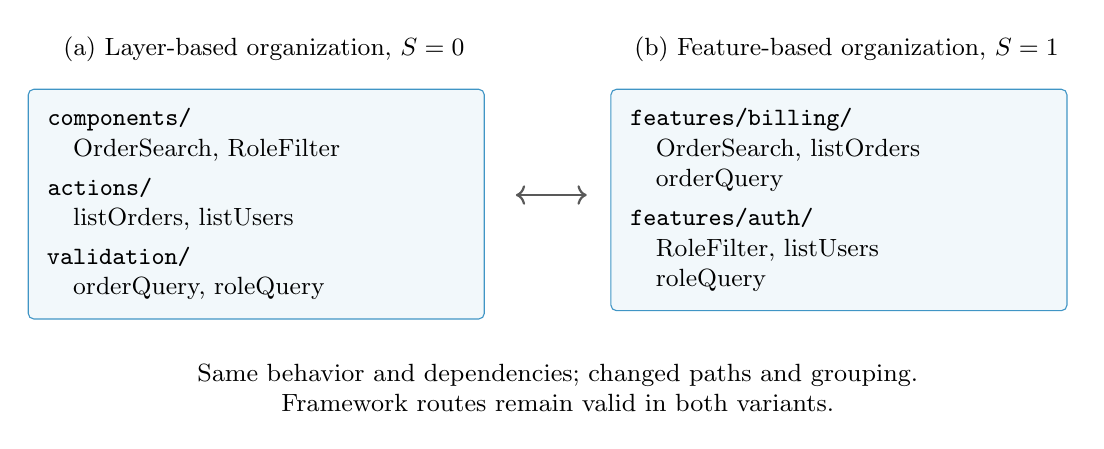
\begin{tikzpicture}
\node[note] at (3,0.5) {(a) Layer-based organization, $S=0$};
\node[note] at (10.4,0.5) {(b) Feature-based organization, $S=1$};
\node[box,text width=5.3cm,anchor=north west,align=left] at (0,0) {\texttt{components/}\\\quad OrderSearch, RoleFilter\\[3pt]\texttt{actions/}\\\quad listOrders, listUsers\\[3pt]\texttt{validation/}\\\quad orderQuery, roleQuery};
\node[box,text width=5.3cm,anchor=north west,align=left] at (7.4,0) {\texttt{features/billing/}\\\quad OrderSearch, listOrders\\\quad orderQuery\\[3pt]\texttt{features/auth/}\\\quad RoleFilter, listUsers\\\quad roleQuery};
\draw[arrow,<->] (6.2,-1.35)--(7.1,-1.35);
\node[note,text width=13cm] at (6.7,-3.8) {Same behavior and dependencies; changed paths and grouping.\\Framework routes remain valid in both variants.};
\end{tikzpicture}
\caption{The organization intervention changes how related source modules are grouped. Names illustrate the planned transformation, not a completed repository refactor or a list of required implementation files. Neither variant is presumed superior.}
\label{fig:organization}
\end{figure}


\subsection{Experimental conditions}
Let $S=0$ denote layer-based organization and $S=1$ feature-based organization. Let $V=0$ denote common basic checks and $V=1$ the same checks plus a behavioral verification package. Figure~\ref{fig:factorial} defines the four conditions and the within-factor comparisons.

\begin{figure}[htbp]
\centering
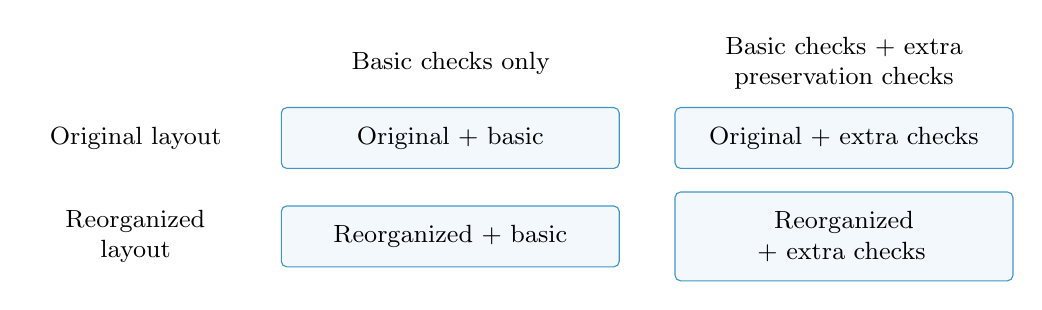
\begin{tikzpicture}
\node[note,text width=4cm] at (4,0.95) {Basic checks only};
\node[note,text width=4cm] at (9,0.95) {Basic checks + extra\\preservation checks};
\node[note,text width=2.5cm] at (0,0) {Original layout};
\node[note,text width=2.5cm] at (0,-1.25) {Reorganized layout};
\node[box,text width=3.8cm] at (4,0) {Original + basic};
\node[box,text width=3.8cm] at (9,0) {Original + extra checks};
\node[box,text width=3.8cm] at (4,-1.25) {Reorganized + basic};
\node[box,text width=3.8cm] at (9,-1.25) {Reorganized + extra checks};
\end{tikzpicture}
\caption{Experimental conditions}
\label{fig:factorial}
\end{figure}


The basic checks will have equivalent invocation and behavioral scope across layouts. Their exact inventory will be recorded during qualification; we will not weaken existing checks to increase the treatment contrast. The additional package will contain runnable checks and controlled fixtures for specified existing behavior, ported to both layouts. Its contents will be fixed before the main experiment. All task requirements will be available in every condition.

Before freezing the intervention, each added check will be mapped to an existing behavioral contract and to a plausible regression that the basic suite does not already detect. Redundant checks may remain for execution convenience, but will not count as additional behavioral coverage. The visible and final suites will use separately authored cases; hidden cases will not be parameter copies of the visible fixtures. A treatment manifest will record files, commands, fixture access, and check runtime in each condition.

The verification intervention supplies executable examples as well as execution feedback. Its estimand is therefore the effect of access to that package. Isolating execution feedback from information content would require an additional control with equivalent information. That question is outside the initial factorial design.

Every condition will receive the same task specification and resource limits. Repository instructions will describe the relevant layout without prescribing superiority or asking the control agent to reconstruct SmartKit's feature organization. Layout-specific path descriptions will be documented. Parent instructions, editor rules, persistent memory, and harness defaults will be controlled, and the instructions actually loaded will be archived. The final evaluator will remain outside the agent workspace.

\subsection{Task construction and provenance}
Tasks will extend an existing application. Each task card will identify its starting snapshot, requirement source, requested behavior, applicable preservation requirements, and intentional changes to existing behavior. Historical issues or pull requests will be preferred when they can be reproduced. Author-constructed tasks will be labeled as such and accompanied by a practical rationale.

The existing task audit contains six constructed candidates, all unvalidated. Figure~\ref{fig:candidate_data} summarizes this actual planning inventory: five candidates concern billing and one concerns administration of user accounts. These counts describe candidate coverage, not agent performance or an admitted benchmark. Qualification must establish that each feature is absent from the starting state, that its requirements are clear, and that feasible correct implementations exist. Task discovery must address the domain imbalance before claiming coverage of the application. Table~\ref{tab:tasks} gives illustrative specifications.

\begin{figure}[!htbp]
\centering
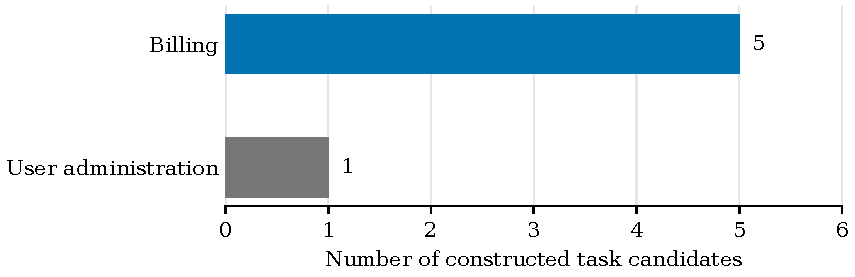
\includegraphics[width=0.92\linewidth]{figures/candidate-data.pdf}
\caption{The current task inventory is concentrated in billing: five of six candidates. Counts are derived from the local task audit; every candidate is author-constructed and unvalidated. They are not experimental observations, and their distribution is not a target allocation for the main study.}
\label{fig:candidate_data}
\end{figure}

\begin{table}[ht]
\small
\renewcommand{\arraystretch}{1.16}
\caption{Constructed task candidates requiring specification and validation.}
\label{tab:tasks}
\begin{tabularx}{\linewidth}{@{}p{0.25\linewidth}YY@{}}
\toprule
Proposed change & Candidate preservation contract & Unresolved specification\\
\midrule
History-page status filter & Retain ownership restrictions and unfiltered behavior & UI contract; existing action filter; empty results\\
Order-code search & Retain ownership checks and payment-code behavior & Exact or prefix matching; case handling\\
Admin role filter & Retain authorization for reading user records & Allowed roles and access policy\\
Batch cancellation & Preserve ownership and state restrictions & Atomic versus partial success\\
\bottomrule
\end{tabularx}
\end{table}

Preservation requirements need support from agreed specifications, existing tests, or confirmed domain rules. The current implementation alone is insufficient when intended behavior is ambiguous. Hidden checks may conceal test inputs, but must not introduce secret business requirements. Changes explicitly authorized by a new task will be excluded from the preservation contract.

A source inspection already refines the status-filter candidate: an existing order-list action accepts a status parameter, whereas the inspected history page queries the signed-in user's orders directly and exposes no filter control. The candidate therefore concerns a history-page interaction and its data path, not inventing backend filtering. The action and page do not currently establish the same access contract; reusing the action without checking authorization could change the page's behavior. These are static source observations, not demonstrated runtime defects. The task remains unqualified until its intended behavior and evaluator are validated.

Task cards, reference solutions, and evaluators will be completed before main runs. Development tasks used to revise the instruments will remain separate from the main task set. Inclusion and exclusion decisions will record their reasons, including ambiguous requirements, inaccessible dependencies, and potential solution leakage through repository history. Agentless's analysis of problematic issue descriptions and exposed ground-truth patches provides a concrete precedent for auditing these risks~\cite{xia2024agentless}.

\subsection{Evaluator qualification}
Each evaluator will check new behavior and preservation independently (Figure~\ref{fig:evaluation}). Before admission, the unchanged baseline must pass preservation checks and fail at least one required acceptance check. A reference patch must pass both groups in each layout. A structurally different valid solution must also be accepted, while plausible faulty implementations must fail the relevant checks. This qualification addresses oracle validity~\cite{barr2015oracle} and test insufficiency~\cite{liu2023evalplus}. Deliberately introduced faults validate the instrument; they are not observations of agent behavior.

Qualification will include repeated executions of unchanged fixtures, valid alternatives, and faulty variants to identify flaky checks. Reviewers will classify failures from task requirements without condition labels where feasible. Evaluator independence means withholding its cases and execution from the agent; it does not remove shared-author bias or make acceptance and preservation statistically independent. Qualification disagreements and the number of checked variants will be reported.

\begin{figure}[htbp]
\centering
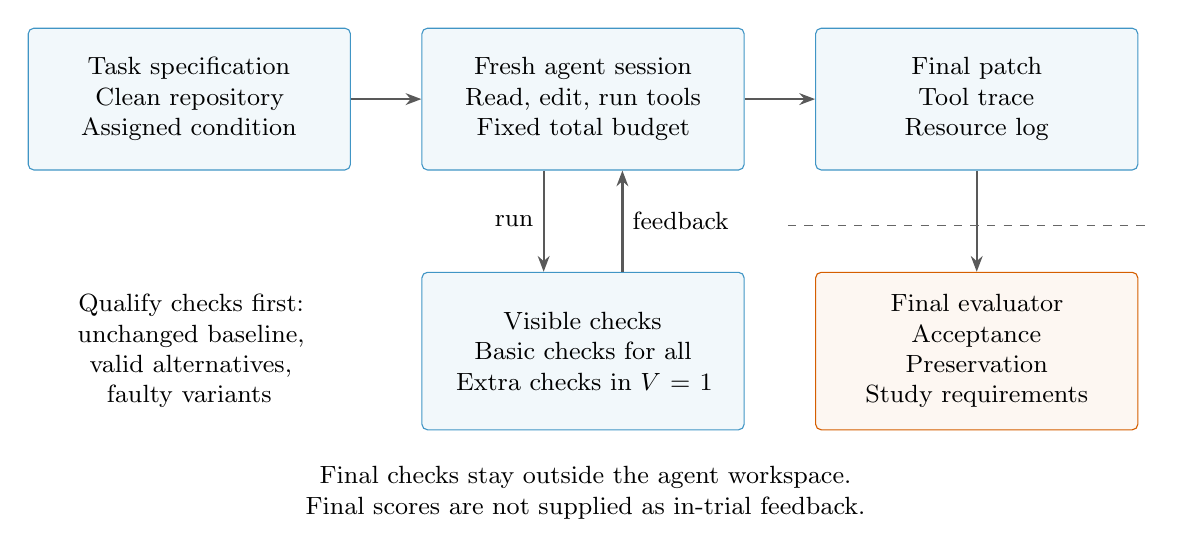
\begin{tikzpicture}
\node[box,text width=3.6cm,minimum height=18mm] (input) at (0,0) {Task specification\\Clean repository\\Assigned condition};
\node[box,text width=3.6cm,minimum height=18mm] (agent) at (5,0) {Fresh agent session\\Read, edit, run tools\\Fixed total budget};
\node[box,text width=3.6cm,minimum height=18mm] (patch) at (10,0) {Final patch\\Tool trace\\Resource log};
\node[box,text width=3.6cm,minimum height=20mm] (visible) at (5,-3.2) {Visible checks\\Basic checks for all\\Extra checks in $V=1$};
\node[box,text width=3.6cm,minimum height=20mm,draw=studyorange,fill=studyorange!5] (hidden) at (10,-3.2) {Final evaluator\\Acceptance\\Preservation\\Study requirements};
\node[note,text width=3.6cm] at (0,-3.2) {Qualify checks first:\\unchanged baseline,\\valid alternatives,\\faulty variants};
\draw[arrow] (input)--(agent);
\draw[arrow] (agent)--(patch);
\draw[arrow] ([xshift=-5mm]agent.south)--node[left,font=\small]{run} ([xshift=-5mm]visible.north);
\draw[arrow] ([xshift=5mm]visible.north)--node[right,font=\small]{feedback} ([xshift=5mm]agent.south);
\draw[arrow] (patch)--(hidden);
\draw[dashed,draw=black!60] (7.6,-1.6)--(12.2,-1.6);
\node[note,text width=13cm] at (5,-5) {Final checks stay outside the agent workspace.\\Final scores are not supplied as in-trial feedback.};
\end{tikzpicture}
\caption{Agents can run the checks supplied in their condition. The same final evaluator scores every saved patch for a given kit and task.}
\label{fig:evaluation}
\end{figure}


Checks will operate at the level needed for the property. Database ownership, uniqueness, and state transitions require suitable integration fixtures. A mock of the persistence operation cannot establish the behavior of the real transaction. Browser or HTTP checks will cover affected interfaces where necessary. Services, data, and clocks will be reset between trials. Payment and email integrations will use controlled fixtures or test environments.

Build and runtime outcomes will be retained separately. A successful build does not establish correct interaction behavior. Conversely, source paths, schema presence, and the number of generated tests will not determine functional success. Agent edits to visible tests cannot change the evaluator's criteria.

\subsection{Allocation and execution}
The experimental unit will be a fresh agent session in an isolated workspace, assigned a task, condition, and fixed model/harness configuration. Conditions will be blocked by task and model/harness, with run order randomized within each block using an archived allocation seed. Every trial will reset application state and agent memory. Repetitions on the same task will remain identified as dependent observations.

For each repetition block, all four conditions will be scheduled in randomized order. Provider outages, execution batch, and any model-version change will be logged; a changed model will define a new configuration rather than silently continuing the same comparison. Reference patches, development solutions, and hidden tests will be removed from reachable repository history and external mounts before agent access. The freeze will specify both wall-time and token limits and a common termination rule. Effects will be interpreted under those limits, including time spent running the verification package.

The main protocol will fix prompts, dependencies, tool permissions, termination rules, and total execution limits. Interface design can affect agent behavior~\cite{yang2024sweagent}, so the harness will be held fixed within each comparison. Verification runs consume the same total budget as other tool use. If several models are feasible, primary estimates will be reported separately for each model/harness. Exact model identifiers, provider versions where available, and execution dates will be recorded.

All attempts will be retained. Agent timeouts and failed implementations will count as outcomes under the allocated budget. Infrastructure failures will follow a separate, predefined adjudication and rerun rule, with original attempts preserved. We will not rerun unsuccessful patches selectively.

\section{Outcomes and analysis plan}
\subsection{Primary and secondary outcomes}
For task $t$, condition $(s,v)$, and repetition $r$, let $A_{tsvr}$ and $P_{tsvr}$ record acceptance and preservation status, respectively. Each is pass, fail, or unassessable. The primary endpoint is
\begin{equation}\label{eq:joint}
Y_{tsvr}=\mathbf{1}\{A_{tsvr}=\mathrm{pass}\ \land\ P_{tsvr}=\mathrm{pass}\}.
\end{equation}
Equation~\eqref{eq:joint} defines joint success. Figure~\ref{fig:outcomes} distinguishes the four possible assessed outcomes without implying their expected frequencies.

\begin{figure}[htbp]
\centering
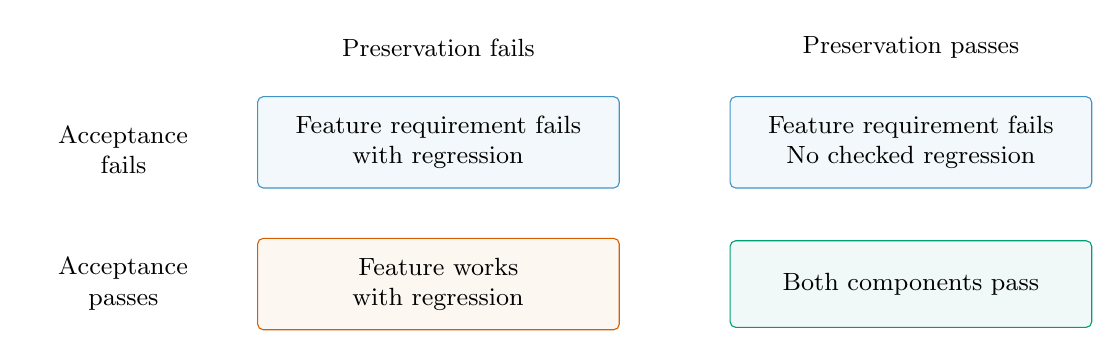
\begin{tikzpicture}
\node[note] at (4,1.2) {Preservation fails};
\node[note] at (10,1.2) {Preservation passes};
\node[note,text width=2.2cm] at (0,-0.1) {Acceptance\\fails};
\node[note,text width=2.2cm] at (0,-1.8) {Acceptance\\passes};
\node[box,text width=4.1cm,minimum height=11mm] at (4,0) {Feature requirement fails\\with regression};
\node[box,text width=4.1cm,minimum height=11mm] at (10,0) {Feature requirement fails\\No checked regression};
\node[box,text width=4.1cm,minimum height=11mm,draw=studyorange,fill=studyorange!5] at (4,-1.8) {Feature works\\with regression};
\node[box,text width=4.1cm,minimum height=11mm,draw=studygreen,fill=studygreen!6] at (10,-1.8) {Both components pass};
\end{tikzpicture}
\caption{Acceptance and preservation outcomes}
\label{fig:outcomes}
\end{figure}

A pass means success within the evaluator's stated scope. An agent-caused build or runtime failure that prevents required behavior from being checked will yield joint failure, with the failure stage recorded. Unassessable components will remain explicit in component summaries. Those summaries will use all attempts with a resolved evaluator outcome as their denominator and separately report pass, fail, and unassessable counts; they will not silently drop unassessable attempts. An independently confirmed infrastructure failure has a missing outcome until the predefined rerun policy resolves it, rather than an assumed agent failure.

Secondary outcomes will include acceptance and preservation results, failure stage, elapsed time, token usage, reported cost, and revision count. We will show the distribution of feature failures and regressions, including cases where the new feature passes but preservation fails. Cost and latency describe agent execution in this setting and will not be converted into estimates of human productivity.

After data collection, the planned result figures will show task-balanced joint success with uncertainty intervals for each condition, paired task-level differences between conditions, and cost distributions including failed attempts. Outcome-category frequencies will distinguish feature failures from regressions. These displays require archived trial data and are not populated in this proposal.

Failure analysis will use evaluator evidence and traces to distinguish omitted behavior, incorrect changes, and failures to use available feedback. A second reviewer, if available, will independently examine a sample under a recorded coding guide. Disagreements and unavailable evidence will remain visible; an LLM-generated explanation alone will not establish a root cause.

\subsection{Contrasts and uncertainty}
Within a model/harness configuration, define the task-balanced success probability over the frozen set of $T$ eligible tasks as
\begin{equation}\label{eq:task_mean}
p_{sv}=\frac{1}{T}\sum_{t=1}^{T}\Pr(Y_{tsvr}=1\mid t,s,v).
\end{equation}
Equation~\eqref{eq:task_mean} gives each task equal weight, regardless of its number of repetitions. We will estimate organization effects at each verification level and verification effects within each organization:
\begin{equation}\label{eq:contrasts}
\Delta_S(v)=p_{1v}-p_{0v},\qquad
\Delta_V(s)=p_{s1}-p_{s0}.
\end{equation}
The additive interaction is
\begin{equation}\label{eq:interaction}
I=(p_{11}-p_{10})-(p_{01}-p_{00}).
\end{equation}
Equations~\eqref{eq:contrasts} and~\eqref{eq:interaction} refer to access to assigned conditions, including trials where an agent never invokes the additional checks. Check use will be a descriptive process outcome, not a condition for inclusion.

For the finite frozen task set, the point estimator is the mean of within-task cell proportions: $\widehat p_{sv}=T^{-1}\sum_t k_{tsv}/n_{tsv}$, where $k_{tsv}$ counts joint successes and $n_{tsv}$ counts attempts with resolved outcomes. A cell with no resolved outcomes will not be dropped and reweighted; collection or adjudication must resolve it, or the planned contrast remains unestimable. Residual missing infrastructure outcomes will be reported by condition with best- and worst-case bounds as a sensitivity analysis.

The two primary intervention summaries will be the equally weighted marginal effects $\overline\Delta_S=\{\Delta_S(0)+\Delta_S(1)\}/2$ and $\overline\Delta_V=\{\Delta_V(0)+\Delta_V(1)\}/2$. Conditional effects and the interaction remain secondary and will be reported together to reveal effect reversal or masking by an average. The main report will emphasize estimates and intervals. If confirmatory tests are retained in the frozen protocol, their family will comprise these two primary effects within the prespecified primary model/harness, with familywise error controlled at 0.05 using Holm's procedure~\cite{holm1979multiple}. Secondary contrasts and additional models will not be promoted to confirmatory claims after outcomes are seen.

Repeated stochastic runs require distribution-aware analysis rather than comparisons of single executions; Arcuri and Briand discuss this issue for randomized software-engineering algorithms~\cite{arcuri2014statistics}. Primary uncertainty will concern repeated agent executions conditional on the frozen tasks. The freeze will select an interval procedure suitable for binary cell outcomes, explicitly handling all-pass and all-fail cells and possible batch dependence. Resampling tasks answers a different question about variation across tasks and will be a secondary sensitivity analysis only, with its exchangeability assumption stated. Constructed convenience tasks do not become a representative random sample because a bootstrap is applied. Closely related task variants will be grouped into families for that analysis. Analyses restricted to patches that build will remain supplementary because that restriction can select different subsets across conditions.

The number of tasks and repetitions is not yet fixed. A separate development pilot will assess evaluator reliability, execution cost, and plausible variability. Before main runs, a precision study will examine plausible baseline success rates, task heterogeneity, boundary cells, and the planned resource limits. Its success criterion will be a prespecified interval width for the primary effects, chosen for a practically meaningful decision rather than copied from a pilot's observed effect. The freeze must settle sample size, interval method, primary model/harness, and missing-outcome policy; until then this is a design proposal, not a confirmatory-ready protocol. More repetitions on a few tasks cannot substitute for task diversity. The interaction will remain exploratory unless its precision is separately justified. A wide interval around a null estimate will not establish equivalence.

\section{Feasibility and reproducibility}
The study is currently at the design stage. Neither the matched layouts nor the candidate tasks have been validated end to end. No fresh pilot or confirmatory data are available. The preceding thesis's pilot artifacts are no longer available and will not be reconstructed from reported scores or reused to estimate intervention effects.

Work will proceed through baseline qualification, task and evaluator construction, matched-condition validation, and a development pilot. The main task set and analysis choices will then be frozen in a dated protocol. Any preregistration must precede inspection of main outcomes. If the variants cannot satisfy the same checked contracts, the organization intervention will be revised before agent comparisons. If prior artifacts already answer the same question, the study will be positioned as a replication or narrowed to a demonstrable extension.

Figure~\ref{fig:data_flow} defines the planned data records and aggregation path. Each attempt will link its task and condition to a versioned environment, loaded instructions, prompts, traces, patch, evaluator outputs, and resource log. Original attempts will remain identifiable after reruns or exclusions. Reference solutions and hidden checks will be separated from agent-accessible material during collection. Release scope will depend on source licenses and permission to redistribute task materials. Test data will replace personal records and service credentials.

\begin{figure}[!htbp]
\centering
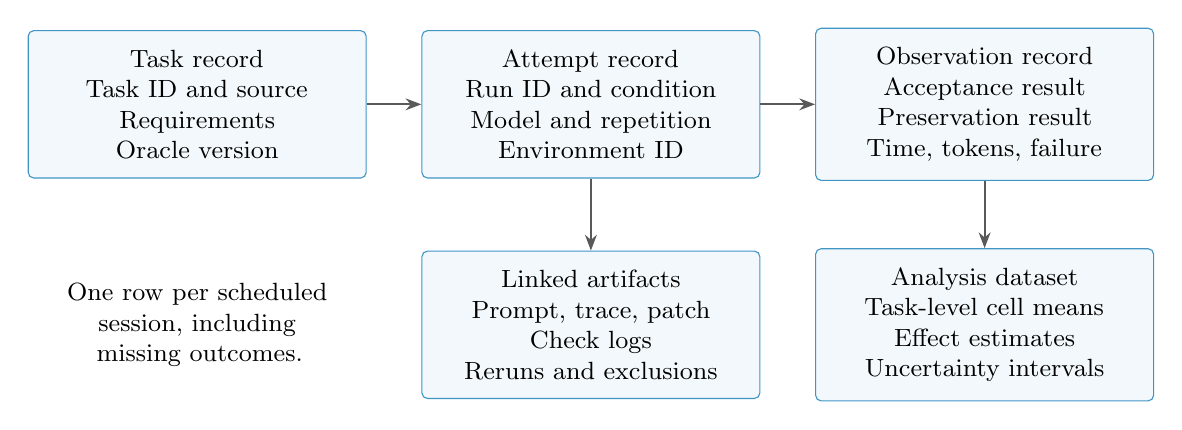
\begin{tikzpicture}[node distance=7mm]
\node[box,text width=3.8cm] (task) at (0,0) {Task record\\Task ID and source\\Requirements\\Oracle version};
\node[box,text width=3.8cm] (run) at (5,0) {Attempt record\\Run ID and condition\\Model and repetition\\Environment ID};
\node[box,text width=3.8cm] (obs) at (10,0) {Observation record\\Acceptance result\\Preservation result\\Time, tokens, failure};
\draw[arrow] (task)--(run);
\draw[arrow] (run)--(obs);
\node[box,text width=3.8cm] (artifact) at (5,-2.8) {Linked artifacts\\Prompt, trace, patch\\Check logs\\Reruns and exclusions};
\node[box,text width=3.8cm] (summary) at (10,-2.8) {Analysis dataset\\Task-level cell means\\Effect estimates\\Uncertainty intervals};
\draw[arrow] (run)--(artifact);
\draw[arrow] (obs)--(summary);
\node[note,text width=3.8cm] at (0,-2.8) {One row per scheduled\\session, including\\missing outcomes.};
\end{tikzpicture}
\caption{Study data and session records}
\label{fig:data_flow}
\end{figure}


\section{Discussion and threats to validity}
The proposed design can estimate the effect of concrete starter-kit interventions within qualified tasks. It cannot establish that feature-based organization is universally preferable. Moving modules changes import paths and the evidence an agent encounters; those changes are part of the intervention. Neutral instructions and a transformation manifest reduce accidental confounding, but do not decompose locality from every other aspect of repository organization.

The verification comparison also has a defined boundary. Its additional tests expose examples and consume execution resources, so a positive result would support the package under the stated budget. It would not identify feedback as the sole cause. An adverse result could arise from execution overhead, distracting examples, or ineffective repair. Trace analysis can help distinguish these explanations without converting them into proven mechanisms.

The author developed SmartKit and will help construct the tasks and evaluator. This creates a risk of favoring familiar paths or requirements. Path-independent outcomes, alternative valid solutions, and independent review where feasible will address specific parts of that risk. Evaluator sensitivity remains limited to the tested contracts, even after these checks.

One repository and a billing-heavy candidate pool limit external validity. Initial conclusions must name the evaluated task set, snapshot, model/harness, and budget. Replication on an independently selected repository would test whether an observed effect transfers beyond SmartKit. A separate human study would be needed to assess maintainability for developers. Neither transfer nor human productivity follows automatically from higher joint success in this experiment.

\section{Conclusion}
We propose a controlled study of repository organization and behavioral verification during agent-driven SaaS feature extension. SmartKit provides an existing application from which matched conditions can be constructed, while independent acceptance and preservation checks define the outcome. The next empirical step is to qualify the baseline and task evaluators. Conclusions about intervention effects will require fresh, fully archived trials under a frozen protocol.

\clearpage
\bibliographystyle{abbrvnat}
\begingroup
\small
\setlength{\bibsep}{4pt}
\raggedright
\bibliography{references}
\endgroup
\end{document}
